\documentclass[11pt,a4paper,draft]{article}
\usepackage[latin1]{inputenc}
\usepackage[margin=1in]{geometry}
\usepackage{amsmath}
\usepackage{amsfonts}
\usepackage{amssymb}
\usepackage{graphicx}
\usepackage{tikz}
\usepackage{pgfplots} 
\pgfplotsset{width=10cm,compat=1.9}
\usepackage{enumitem}

\setlength\abovedisplayskip{0pt}
\author{James Brissette}
\title{CS-6210: HW 1}

\begin{document}
		\maketitle
	
	\section{Chapter 3: Questions 6,12,16,24,25}
	\begin{itemize}
		\item [3.6]
		\begin{enumerate} [label={\alph*)}]
			\item Here I solve for $A^{-1}$ the old school way:
			$$
			\begin{array}{cc}
				\left(\begin{array}{ccc|ccc}
				1 & 1 & 0 & 1 & 0 & 0 \\
				0 & 1 & 1 & 0 & 1 & 0 \\
				1 & 0 & 1 & 0 & 0 & 1 \\
				\end{array}
				\right) \rightarrow &
				
				\left(
				\begin{array}{ccc|ccc}
				1 & 1 & 0 & 1 & 0 & 0 \\
				0 & 1 & 1 & 0 & 1 & 0 \\
				0 & -1 & 1 & -1 & 0 & 1 \\
				\end{array}
				\right) \rightarrow \\
				
				R3-R1\rightarrow R3 & R1-R2\rightarrow R1 \\ \\
				
				\left(
				\begin{array}{ccc|ccc}
				1 & 0 & -1 & 1 & -1 & 0 \\
				0 & 1 & 1 & 0 & 1 & 0 \\
				0 & -1 & 1 & -1 & 0 & 1 \\
				\end{array}
				\right) \rightarrow &
				
				\left(\begin{array}{ccc|ccc}
				1 & 0 & -1 & 1 & -1 & 0 \\
				0 & 1 & 1 & 0  & 1 & 0 \\
				0 & 0 & 2 & -1 & 1 & 1 \\
				\end{array}
				\right) \rightarrow	\\
				
				R3+R2\rightarrow R3 & R3/2\rightarrow R3 \\ \\
				
				\left(\begin{array}{ccc|ccc}
				1 & 0 & -1 & 1 & -1 & 0 \\
				0 & 1 & 1 & 0  & 1 & 0 \\
				0 & 0 & 1 & -\frac{1}{2} & \frac{1}{2} & \frac{1}{2} \\
				\end{array}
				\right) \rightarrow &
				
				\left(
				\begin{array}{ccc|ccc}
				1 & 0 & 0 & \frac{1}{2} & -\frac{1}{2} & \frac{1}{2} \\
				0 & 1 & 0 & \frac{1}{2} & \frac{1}{2} & -\frac{1}{2} \\
				0 & 0 & 1 & -\frac{1}{2} & \frac{1}{2} & \frac{1}{2} \\
				\end{array}
				\right) \\
				
				Solve & 
			\end{array}
			$$
			\item 
			$$\vert\vert A \vert\vert = \max (2,2,2) = 2$$ 
			$$\vert\vert A^{-1} \vert\vert = \max (\frac{3}{2},\frac{3}{2},\frac{3}{2}) = \frac{3}{2}$$
			$$k_\infty(A) = \vert\vert A \vert\vert * \vert\vert A^{-1} \vert\vert = 3$$ 
			\item
			$$\begin{pmatrix}
				1 & 1 & 0 \\
				0 & 1 & 1 \\
				1 & 0 & 1 \\
			\end{pmatrix} = 
			\begin{pmatrix}
			1 & 0 & 0 \\
			l_{12} & 1 & 0 \\
			l_{13} & l_{23} & 1 \\
			\end{pmatrix}
			\begin{pmatrix}
			u_{11} & u_{21} & u_{31} \\
			0 & u_{22} & u_{32} \\
			0 & 0 & u_{33} \\
			\end{pmatrix} $$
			$$= \begin{pmatrix}
			u_{11} & u_{21} & u_{31} \\
			u_{11}l_{12} & u_{21}l_{12}+u_{22} & u_{31}l_{12}+u_{32} \\
			u_{11}l_{13} & u_{21}l_{13}+u_{22}l_{23} & u_{31}l_{13}+u_{32}l_{23}+u_{33} \\
			\end{pmatrix} $$
			Solving for each unknown we get:
			$$ \begin{array}{ccc}
					u_{11} = 1 & u_{21} = 1  & u_{31} = 0 \\
					l_{12} = 0 & u_{22} = 1  & u_{32} = 1 \\
					l_{13} = 1 & l_{23} = -1 & u_{33} = 2
				\end{array}
			$$ And the Doolittle factorization becomes:
			$$ \begin{pmatrix}
			1 & 0 & 0 \\
			0 & 1 & 0 \\
			1 & -1 & 1 \\
			\end{pmatrix}
			\begin{pmatrix}
			1 & 1 & 0 \\
			0 & 1 & 1 \\
			0 & 0 & 2 \\
			\end{pmatrix} $$
		\end{enumerate}
	
		\item [3.12]
		\begin{enumerate} [label={\alph*)}]
			\item To determine the values $\alpha$ that make $A$ \textit{ill-conditioned}, we can compute the condition number $k$ using the infinity norm, denoted $k_\infty$:
			$$
			\begin{array}{ccc} 
				A = \begin{pmatrix} -1 & 1 \\ 0 & \alpha \end{pmatrix} & & A^{-1}=\begin{pmatrix} -1 & 1/\alpha \\ 0 & 1/\alpha \end{pmatrix} \\
				\vert\vert A \vert\vert = \max(2,\alpha) & & \vert\vert A^{-1} \vert\vert = 1+\frac{1}{\alpha}
			\end{array}
			$$
			%
			The condition number can then be computed as:
			$$k_\infty(A) = \vert\vert A \vert\vert * \vert\vert A^{-1} \vert\vert$$
			
			For $0 < \alpha \leq 2$, $k$ takes the values:  $2*(\frac{1+\alpha}{\alpha})$; and for $2 < \alpha$, $k$ can be calculated as:  $1+\alpha$. This is most easily seen as we graph the curve for both domains of $\alpha$:
			$$
				\begin{tikzpicture}
				\begin{axis}[
					xtick={0,2,5,10,15,20}
				]
				\addplot[domain=0:2,red] {2+2/x};
				\addplot[domain=2:20,blue] {1+x};
				\end{axis}
				\end{tikzpicture}
			$$	
			The matrix $A$ will be ill-conditioned for very small values of $\alpha$ ($0 < \alpha \ll 1$) and for very large values of $\alpha$ ($k$ increases linearly with $\alpha$).
			
			\item Error can also be defined as $e=A^{-1}r$, which is convenient considering $\alpha$ is an element of the matrix $A$. In that case $e_1=-r_1+\frac{r_2}{\alpha}$ and $e_2=\frac{r_2}{\alpha}$. It quickly becomes apparent that a matrix $A$ which contains very small ($\alpha \ll 1$) values of $\alpha$ could take a small residual and create a large error.
			
			\item Conversely, residual can be written as $r=Ae$, which allows us to see the effect of $\alpha$ on $r$. Here we see $r_1=-e_1+e_2$ and $r_2=\alpha e_2$. The effect of $\alpha$ on error is opposite, where $r$ can be large given a small $e$ if $\alpha \gg 1$.
		\end{enumerate}
	
		\item [3.16]
			\begin{enumerate}
				\item Need to solve in MATLAB
			\end{enumerate}
		
		\item [3.24] $ $
			\begin{enumerate} [label={\alph*)}]
				%Part A of Question 3.24
				\item Based solely on the sketch, the solutions are located (approximately) at ($x_1=.85$) and ($x_2=2$):\\ 
				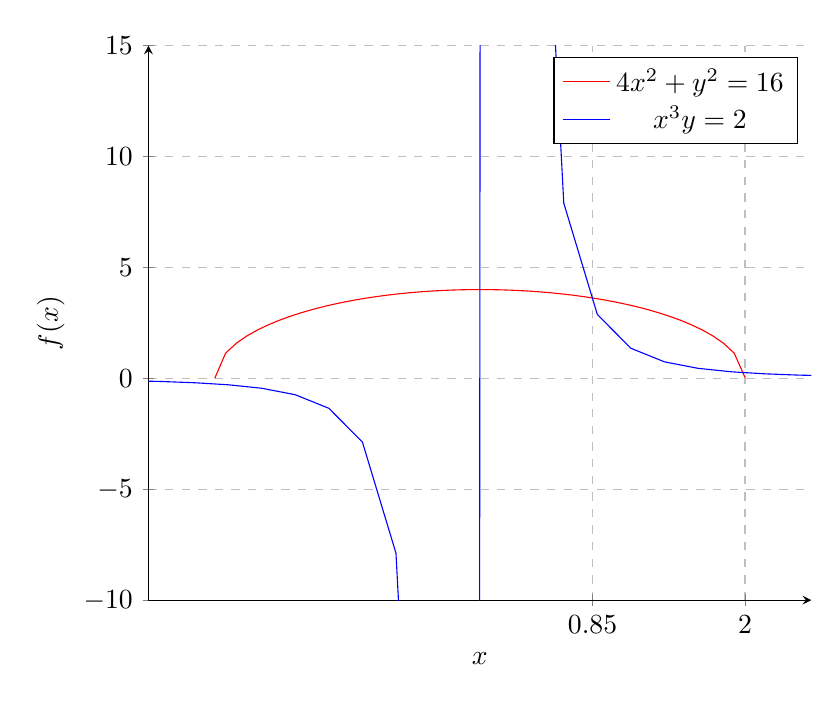
\begin{tikzpicture}
				\begin{axis}[
				axis lines = left,
				xlabel = $x$,
				ylabel = {$f(x)$},
				xmin= -2.5, xmax = 2.5,
				ymin = -10, ymax =15,
				xtick = {.85,2},
				ymajorgrids=true,
				xmajorgrids=true,
				grid style=dashed
				]
				%
				\addplot [
				domain=-2:2, 
				samples=50, 
				color=red,
				]
				{sqrt(16-4*x^2)};
				\addlegendentry{$4x^2 + y^2 = 16$}
				%
				\addplot [
				domain=-10:10, 
				samples=80, 
				color=blue,
				]
				{2 / x^3};
				\addlegendentry{$x^3y=2$}
				
				\end{axis}
				\end{tikzpicture}
				
				%Part B of Question 3.24
				\item Calculating the Jacobian matrix $J$ of the nonlinear system of equations involves taking the partial derivatives of each equation with respect to $x$ and $y$:
				%
				$$\begin{bmatrix} f(x,y) \\ g(x,y) \end{bmatrix} = \begin{bmatrix} 4x^2+y^2-16 \\ x^3y-2 \end{bmatrix}$$
				%
				$$J = \begin{bmatrix} 8x & 2y \\ 3x^2y & x^3 \end{bmatrix} and\ f = \begin{bmatrix} 4x^2+y^2-16 \\ x^3y-2 \end{bmatrix} $$\
				%
				
				\item Good initial starting values for the solutions, again going based off the sketch, would be anywhere in the general range of the expected solution. A convention that appears to be common (I could be mistaken) is to choose an easy to calculate point like $x=1$. I would guess, given the curves, that wouldn't be a bad place to begin here either. After 2 or 3 iterations, you would have a good approximation of either solution depending on which curve you plugged $x$ into initially. In fact, any initial starting value of $x$ where $x > 0$ seems like it would work if you began with the blue curve, and any point $0 < x < 2$ if starting with the red curve.
				
			\end{enumerate}
		\item [3.25] $ $
			\begin{enumerate} [label={\alph*)}]
				%Part A of Question 3.25
			\item The algorithm works only because of the combination of the simplified and generalizable LU factorization of tri-diagonal matricies and the convenience of Cholesky Factorization. Factorizations of tri-diagonal matrices take the form:
			%
			$$\begin{pmatrix}
				l_{11} &        &        &        &            &        \\ 
				l_{12} & l_{22} &        &        &            &        \\
				       & l_{23} & l_{33} &        &            &        \\
				       &        & \ddots & \ddots &            &        \\
				       &        &        &        &            &        \\
			           &        &        &        & l_{i-1,i}  & l_{ii}
			\end{pmatrix}
			\begin{pmatrix}
			u_{11} & u_{21} &        &        &        &            \\ 
			       & u_{22} & u_{32} &        &        &            \\
			       &        & u_{33} & u_{43} &        &            \\
		           &        &        & \ddots & \ddots &            \\
			       &        &        &        &        & u_{i,i-1}  \\
			       &        &        &        &        & u_{ii}
			\end{pmatrix}
			$$
			%
			And Cholesky allows us to simplify the process by assuming $A=U^TU$ rather than $A=LU$ by setting $L=U^T$. This allows our factorization to become:
			%
			$$\begin{pmatrix}
			u_{11} &        &        &        &            &        \\ 
			u_{21} & u_{22} &        &        &            &        \\
			       & u_{32} & u_{33} &        &            &        \\
				   &        & \ddots & \ddots &            &        \\
				   &        &        &        &            &        \\
				   &        &        &        & u_{i,i-1}  & u_{ii}
			\end{pmatrix}
			\begin{pmatrix}
			u_{11} & u_{21} &        &        &        &            \\ 
				   & u_{22} & u_{32} &        &        &            \\
				   &        & u_{33} & u_{43} &        &            \\
				   &        &        & \ddots & \ddots &            \\
				   &        &        &        &        & u_{i,i-1}  \\
				   &        &        &        &        & u_{ii}
			\end{pmatrix}
			$$
			%
			Where the super/sub diagonals have the same values. Combining the matrices, you come to the general form:
			%
			$$\begin{pmatrix}
			u^2_{11}     &     u_{11}u_{21}   &                    &        &                  &                    \\ 
			u_{11}u_{21} &   u^2_{21}u^2_{22} &    u_{22}u_{32}    &        &                  &                     \\
			             &     u_{22}u_{32}   &  u^2_{32}u^2_{33}  &        &                  &                     \\
			             &                    &      \ddots        & \ddots &     \ddots       &                     \\
		 	             &                    &        			   &        &                  &  u_{ij}u_{i+1,j}     \\
			             &                    &       			   &        & u_{ij}u_{i+1,j}  & u^2_{i,j-1}u^2_{ij}
			\end{pmatrix}
			$$
			%
			It then becomes apparent that the algorithm solves this factorization. The upper-leftmost value $u^2_{11}$ (or $d^2_1$ in the algorithm) equals the upper-leftmost value in the original tridiagonal matrix, $a_1$. And solving for $d_1$ we see $d_1 = \sqrt{a_1}$. The rest is equally trivial to connect if we remember that $L=U^T$ and so $u_{i,i+1} = u_{i+1,i}$ for every entry along the super/sub diagonal, and to fill in the blanks in the algorithm, $v_{i-1} = \frac{b_{i-1}}{d_{i-1}}$, where $b_{i-1}$ is the subdiagonal entry $b$ at index $i$ in the original matrix $A$; $d_i$ is then calculated by solving:
			$$v^2_{i-1}d^2_i = a_i$$ $$d_i = \sqrt{a_i}/v_{i-1}$$
			
			\item The equation needs to be solved in two parts: First, we solve $U^Ty = z$. Second, using our answer for $y$, we calculate $Ux=y$. The first part of the algorithm solves for $y$, by first calculating the trivial case where $d_1y_1=z_1$ (because the upper diagonal of $U^T$ is zero) $\rightarrow$ $y_1 = z_1/d_1$.\\ The remaining $y$'s can be solved by calculating $v_{i-1}y_{i-1}+d_iy_i=z_i$. For $i = 2:n$, $y_i=(z_i-y_{i-1}v_{i-1})/d_i$. \\
			Once $y$ has been calculated, we solve for $x$ via the equation $Ux=y$. It's important to remember the matrix $U$ is upper diagonal with values on the main diagonal, super diagonal and zeros everywhere else. The trivial case here is no longer located at $d_1$, but at $d_n$ where $d_nx_n=y_n$. The algorithm takes this into account by first solving $x_n=y_n/d_n$ and then backsolving the remaining $x$'s: $$d_nx_n + d_{n-1}x_{n-1} = y_{n-1}$$ $$x_{n-1} = (y_{n-1}-d_nx_n)/d_{n-1}$$ Or for the arbitrary case $i$ for $i = n-1:1 \rightarrow x_{i} = (y_{i}-d_{n+1}x_{i+1})/d_{i}$
			
			\item Need MATLAB
			\item
			\end{enumerate}
			
	\end{itemize}
	
	\section{Chapter 4: Questions 10,22,31}
	\begin{itemize}
		\item [4.10]
		
		\item [4.22]
		
		\item [4.31]
	\end{itemize}
	
	
\end{document}